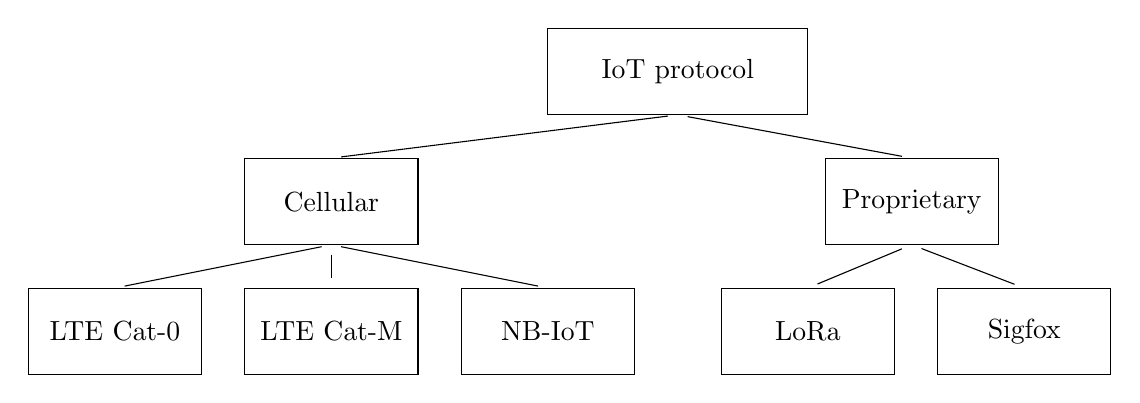
\begin{tikzpicture}[scale=0.11]
\draw  (10,100) rectangle (40,90);
\node at (25,95) {IoT protocol};
\draw  (-25,85) rectangle (-5,75);
\node at (-15,80) {Cellular};
\draw  (42,85) rectangle (62,75);
\node at (52,80) {Proprietary};

\draw  (-50,70) rectangle (-30,60);
\node at (-40,65) {LTE Cat-0};
\draw  (-25,70) rectangle (-5,60);
\node at (-15,65) {LTE Cat-M};
\draw  (0,70) rectangle (20,60);
\node at (10,65) {NB-IoT};
\draw  (30,70) rectangle (50,60);
\node at (40,65) {LoRa};
\draw  (55,70) rectangle (75,60);
\node at (65,65) {Sigfox};


%\draw  (-2,47) ellipse (4 and 4);
%\draw (-2,51) -- (48,51) -- (48,43) -- (-2,43);
%\node at (-2,47) {A};
%\node [anchor=west] at (8,47) {Reliability};
%
%\draw  (-2,35) ellipse (4 and 4);
%\draw (-2,39) -- (48,39) -- (48,31) -- (-2,31);
%\node at (-2,35) {B};
%\node [anchor=west] at (8,35) {Energy consumption};
%
%\draw  (-2,23) ellipse (4 and 4);
%\draw (-2,27) -- (48,27) -- (48,19) -- (-2,19);
%\node at (-2,23) {C};
%\node [anchor=west] at (8,23) {Massiveness};

\node (v1) at (25,90) {};
\node (v2) at (-15,85) {};
\node (v3) at (52,85) {};
\node (v4) at (-15,75) {};
\node (v5) at (-40,70) {};
\node (v6) at (-15,70) {};
\node (v7) at (10,70) {};
\node (v8) at (52,75) {};
\node (v9) at (40,70) {};
\node (v10) at (65,70) {};
\draw  (v1) edge (v2);
\draw  (v1) edge (v3);
\draw  (v4) edge (v5);
\draw  (v4) edge (v6);
\draw  (v4) edge (v7);
\draw  (v8) edge (v9);
\draw  (v8) edge (v10);
\end{tikzpicture}